% TikZ code for KST proof sketch, v7 (1-indexed)
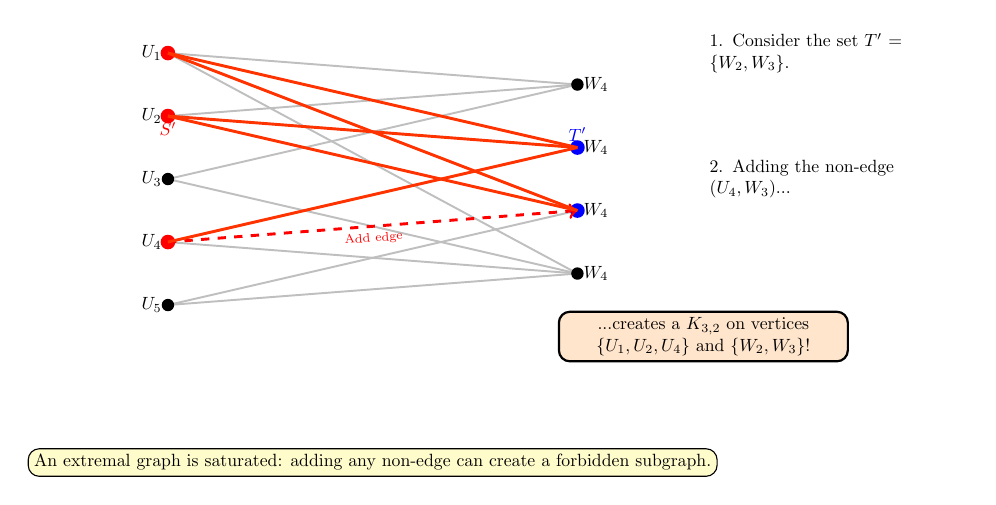
\begin{tikzpicture}[scale=0.8, every node/.style={transform shape, scale=0.8}]
\pgfdeclarelayer{background}
\pgfdeclarelayer{main}
\pgfsetlayers{background,main}
\coordinate (U0) at (0, 4.0);
\coordinate (U1) at (0, 3.0);
\coordinate (U2) at (0, 2.0);
\coordinate (U3) at (0, 1.0);
\coordinate (U4) at (0, 0.0);
\coordinate (W0) at (6.5, 3.5);
\coordinate (W1) at (6.5, 2.5);
\coordinate (W2) at (6.5, 1.5);
\coordinate (W3) at (6.5, 0.5);
\begin{pgfonlayer}{main}
\uncover<1->{
  \draw[line width=0.7pt, black!25] (U0) -- (W0);
  \draw[line width=0.7pt, black!25] (U0) -- (W1);
  \draw[line width=0.7pt, black!25] (U0) -- (W2);
  \draw[line width=0.7pt, black!25] (U0) -- (W3);
  \draw[line width=0.7pt, black!25] (U1) -- (W0);
  \draw[line width=0.7pt, black!25] (U1) -- (W1);
  \draw[line width=0.7pt, black!25] (U1) -- (W2);
  \draw[line width=0.7pt, black!25] (U2) -- (W0);
  \draw[line width=0.7pt, black!25] (U2) -- (W3);
  \draw[line width=0.7pt, black!25] (U3) -- (W1);
  \draw[line width=0.7pt, black!25] (U3) -- (W3);
  \draw[line width=0.7pt, black!25] (U4) -- (W2);
  \draw[line width=0.7pt, black!25] (U4) -- (W3);
  \fill[black] (U0) circle (2.8pt) node[anchor=east] {$U_{1}$};
  \fill[black] (U1) circle (2.8pt) node[anchor=east] {$U_{2}$};
  \fill[black] (U2) circle (2.8pt) node[anchor=east] {$U_{3}$};
  \fill[black] (U3) circle (2.8pt) node[anchor=east] {$U_{4}$};
  \fill[black] (U4) circle (2.8pt) node[anchor=east] {$U_{5}$};
  \fill[black] (W0) circle (2.8pt) node[anchor=west] {$W_{4}$};
  \fill[black] (W1) circle (2.8pt) node[anchor=west] {$W_{4}$};
  \fill[black] (W2) circle (2.8pt) node[anchor=west] {$W_{4}$};
  \fill[black] (W3) circle (2.8pt) node[anchor=west] {$W_{4}$};
  \node[draw, fill=yellow!20, rounded corners, align=center] at (3.25, -2.5) {An extremal graph is saturated: adding any non-edge can create a forbidden subgraph.};
}
\uncover<2->{
  \node[blue, anchor=south, font=\bfseries] at (W1) {$T'$};
  \fill[blue] (W1) circle (3.3pt);
  \fill[blue] (W2) circle (3.3pt);
  \node[anchor=west, text width=4cm, align=left] at (8.5, 4) {1. Consider the set $T' = \{W_2, W_3\}$.};
  \fill[red] (U0) circle (3.3pt);
  \fill[red] (U1) circle (3.3pt);
  \fill[red] (U3) circle (3.3pt);
  \node[red, anchor=north, font=\bfseries] at (U1) {$S'$};
  \draw[line width=1.0499999999999998pt, red, dashed, ->] (U3) -- (W2) node[midway, below, sloped, font=\scriptsize] {Add edge};
  \node[anchor=west, text width=5cm, align=left] at (8.5, 2.0) {2. Adding the non-edge $(U_4, W_3)$...};
  \draw[line width=1.0499999999999998pt, red!60!orange] (U0) -- (W1);
  \draw[line width=1.0499999999999998pt, red!60!orange] (U0) -- (W2);
  \draw[line width=1.0499999999999998pt, red!60!orange] (U1) -- (W1);
  \draw[line width=1.0499999999999998pt, red!60!orange] (U1) -- (W2);
  \draw[line width=1.0499999999999998pt, red!60!orange] (U3) -- (W1);
  \node[draw, fill=orange!20, rounded corners, align=center, thick, text width=5.5cm] at (8.5, -0.5) {...creates a $K_{3,2}$ on vertices \\ $\{U_1, U_2, U_4\}$ and $\{W_2, W_3\}$!};
}
\end{pgfonlayer}
\end{tikzpicture}